\documentclass{article}

\usepackage[utf8]{inputenc} % un package
\usepackage[T1]{}      % un second package
\usepackage[francais]{babel}  % un troisième package
\usepackage{fancyhdr}
\usepackage{wrapfig}
\usepackage{graphicx}
\usepackage[left=2cm, right=2cm]{geometry}

\title{Rapport de stage}
\author{Chadi \bsc{AKEL}}
\date{\today}

\begin{document}
\pagestyle{fancy}
\lhead{\thepart}
\chead{}
\lfoot{}
\cfoot{\thepage}
\rfoot{}
\maketitle
\newpage
\rhead{Sommaire}
\renewcommand{\contentsname}{Sommaire}
\tableofcontents

\newpage
\rhead{Remerciements}
\part{Remerciements}
	Avant tout développement sur cette expérience professionnelle, il apparaît opportun de commencer ce rapport de stage par des remerciements, 
	à ceux qui m'ont beaucoup appris au cours de ce stage, et même à ceux qui ont eu la gentillesse de faire de ce stage un moment très profitable. 
	Aussi, je remercie touts les membres de l'équipe, et plus particulirement Gaetan Bayle et Jean-François Lemerre, qui m'ont formés et accompagnés 
	tout au long de cette expérience professionnelle avec beaucoup de patience et de pédagogie. Enfin, je remercie l'ensemble des employés de bull 
	pour les conseils qu'ils ont pu me prodiguer au cours de ces six mois.

\newpage
\rhead{Introduction}
\part{Introduction}
	Du 1er Avril au 30 Septembre 2012, j’ai effectué un stage au sein de l’entreprise Bull située au Clayes-sous-bois 
	dans les Yvelines. Bull étant un acteur important dans le domaine du calcul haute performance, j'ai naturellement 
	était très enthousiaste à l'idée d'y faire mon stage. Le poste proposé permettait d'étudier les performances de 
	l'accélerateur d'Intel (MIC) et d'autres GPUs de Nvidia ou AMD. Il était aussi question de travailler sur le projet 
	OpenGPU en partenariat avec l'école centrale de Paris. Ce stage correspondait donc parfaitement à ma formation et 
	l'étude des performances est un domaine que j'apprécie et sur lequel j'ai aussi eu l'occasion de travailler lors de 
	mon précedent stage au laboratoire Exascale.
	[Ici présenter de maniere globale l'entreprise qui sera plus détaillé dans la partie 1]
	Au cours de ce stage au département R\&D dans l'équipe performance, j’ai pu m’intéresser aux accélérateurs tel que les GPU... 
	[parler rapidement de la mission de mon stage qui sera plus détaillée dans la partie 2]

\newpage
\rhead{L'entreprise et son secteur d'activité}
\part{L'entreprise et son secteur d'activité}
	\section{L'entreprise}
		\subsection{Historique}
		\begin{center}
		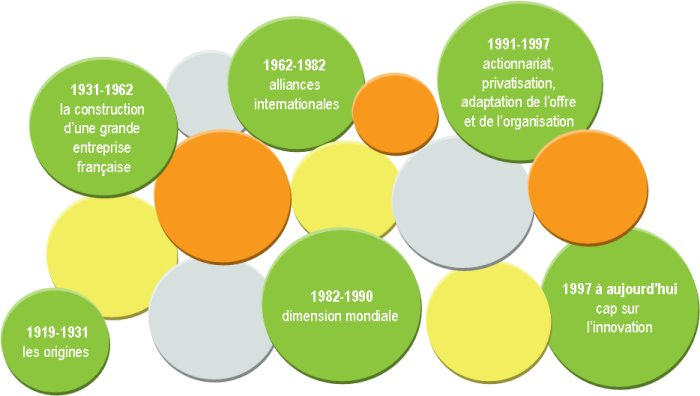
\includegraphics[scale=0.5]{histoire_fr.jpg}
		\end{center}
		\subsubsection{1919-1931: les origines}
		\paragraph{}
		\begin{bf}1919\end{bf} : L’ingénieur norvégien Fredrik Rosing Bull a pour défi de concevoir 
		\begin{wrapfigure}[8]{l}{3cm}
		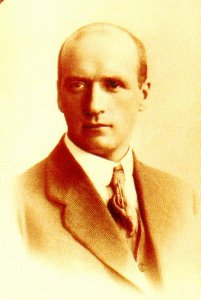
\includegraphics[scale=0.75]{FredrikRosingBull.jpg}
		\caption{Fredrik Rosing Bull 1882-1925}
		\end{wrapfigure}
		une machine d’automatisation du traitement de statistiques pour la compagnie d’assurance Storebrand, qui est son employeur. 
		En août \begin{bf}1921\end{bf}, le prototype est présenté au conseil d'administration de Storebrand qui l'adopte. 
		La presse spécialisée fait une bonne publicité à la machine de F.R. Bull. Une demi-douzaine d'exemplaires est livrée à diverses entreprises 
		entre \begin{bf}1922\end{bf} et \begin{bf}1925\end{bf}. Ce succès est dû à la fois aux qualités techniques de la 
		machine (notamment à sa simplicité) et au fait que son apparition met fin à l'emprise du système Hollerith (IBM), 
		faisant ainsi baisser les prix et donnant le choix aux clients.
		\newline{}
		\newline{}
		\newline{}
		\newline{}
		\newline{}
		\newline{}
		\newline{}
		\newline{}
		\paragraph{}
		A la mort de F.R. en \begin{bf}1925\end{bf}, l'initiateur principal de l'expansion européenne de Bull est Émile 
		Genon, un belge qui vendait des machines à calculer. Il achète en \begin{bf}1927\end{bf} les droits relatifs aux 
		brevets de F.R. Bull pour dix pays d'Europe. Il entraîne la société H.W. Egli, établie en Suisse, à acquérir en \begin{bf}1928\end{bf}
		 les droits industriels touchant ces brevets hors des pays scandinaves et les machines sont fabriquées en Suisse dès \begin{bf}1928\end{bf}.
		\paragraph{}
		En décembre \begin{bf}1929\end{bf} la \begin{bf}première machine\end{bf} fabriquée à Zürich est livrée aux laboratoires Sandoz. 
		La recherche d’un marché national fort, capable d’absorber une production de type industriel, ainsi que la législation 
		protégeant les brevets l’a conduit à s’implanter en France.
		\paragraph{}
		\begin{bf}1931\end{bf}: En mars 1931 à Paris, la société H.W. Egli Bull, de droit français mais à majorité suisse, 
		est fondée par trois partenaires : la société suisse H.W. Egli, la société Bull AG fondée l'année précédente à Zürich 
		par Genon et enfin l'ATEIC (Association Technique d'Études industrielles et Comptables). Elle \begin{bf}vendra les 
		machines Bull en France\end{bf}. Elle s’installe avenue Gambetta dans le 20eme arrondissement de Paris ; le site est 
		aujourd’hui occupé par le rectorat de l’académie de Paris.
		\subsubsection{1931-1962: la construction d'une grande entreprise française}
		\paragraph{}
		\begin{bf}1931\end{bf}: Les études de Bull, sous la direction de Knut Andréas Knutsen, sortent la tabulatrice T30,
		\begin{wrapfigure}[8]{l}{3cm}
		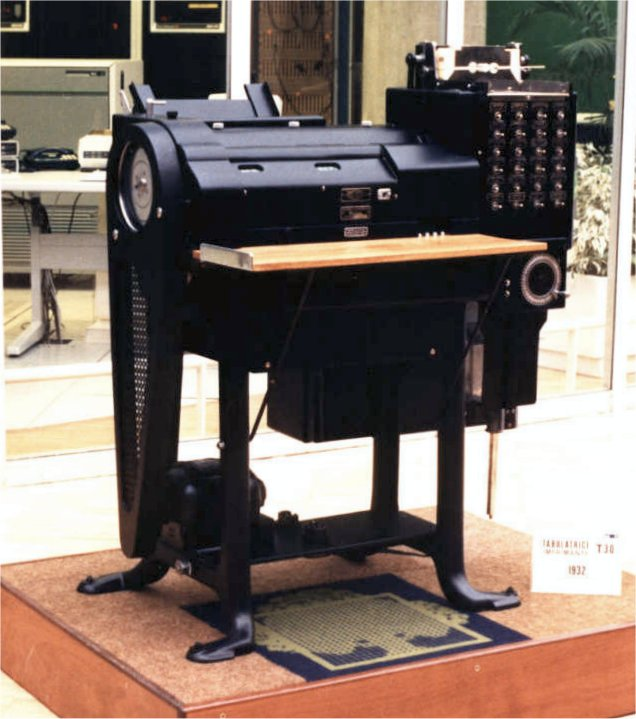
\includegraphics[scale=0.25]{tabulatrice_t30.jpg}
		\caption{Tabulatrice T30}
		\end{wrapfigure}
		25 à 40\% moins chère que la concurrence et capable d’imprimer 120 lignes à la minute. Un record mondial, \begin{bf}qui 
		ne sera égalé que dix-huit ans plus tard\end{bf}! Cette performance est à l’origine du développement commercial de Bull.
		\newline{}
		\newline{}
		\newline{}
		\newline{}
		\newline{}
		\newline{}
		\newline{}
		\newline{}
		\paragraph{}
		\begin{bf}1933\end{bf}: Création de la \begin{bf}CMB\end{bf} (Compagnie des Machines Bull). Née des brevets de machines 
		mécanographiques de Frederik Rosing Bull et Knut Andréas Knutsen, elle a succédé à la société franco-suisse Egli-Bull. 
		Deux ans plus tard (1935), elle détient 16\% du marché français, devient le principal concurrent d'IBM en France et 
		est commercialisée en Belgique, Suisse, Italie, Argentine et les pays Scandinaves. Sa tabulatrice est une des 
		meilleures du marché et la plus rapide. Technologiquement, la CMB ne cesse d’innover. Elle jouit d’une excellente 
		réputation de rapidité et de richesse fonctionnelle, et est bien adaptée aux applications européennes. L’entreprise 
		construit environ trois équipements par mois et augmente régulièrement sa capacité de production.
		\paragraph{}
		\begin{bf}1935\end{bf}: L'innovation exigeant des investissements coûteux, des pourparlers sont entrepris avec les 
		pouvoirs publics en vue d'obtenir une aide pour le développement des études. E. Genon est mandaté par le Conseil 
		d'Administration afin de poursuivre auprès de différentes firmes aux États-Unis les recherches d'accords de licence et 
		de distribution. Il rencontre IBM qui lui fait une offre de collaboration amicale. Mais la compagnie préfère demander 
		l'engagement du gouvernement français, dont la décision tarde à venir. Genon, sans avoir reçu l'autorisation du conseil 
		d'administration, vend alors à IBM la majorité des actions de Bull A.G. (la société de commercialisation des machines 
		Bull, qu'il dirigeait). Il y voit un moyen d'obtenir « une paix tacite » des brevets entre IBM et Bull et de 
		développer Bull sur le plan international avec l'appui d'un groupe américain. L'intraitable Georges Vieillard, alors 
		Directeur de la CMB somme Genon de choisir : Bull ou IBM. \begin{bf}Après dix ans d'une intense activité souvent décisive,\end{bf} 
		Genon quitte Bull. De nouveaux acteurs entrent en scène : la famille Callies-Aussedat.
		\paragraph{}
		La Société des Papeteries Aussedat fournissait Bull en cartes mécanographiques utilisées par les machines. Depuis 
		1932, elle avait réalisé d'importants investissements dans ce domaine et était représentée au Conseil d'Administration 
		de Bull par Jacques Callies. La menace d'une absorption de la compagnie par IBM inquiétait Aussedat car IBM exigeait 
		de ses clients qu'ils lui achètent les cartes en exclusivité.
		\paragraph{}
		De même qu'il fallait éviter le rachat de Citroën par General Motors, il ne fallait pas que la Compagnie des Machines 
		Bull tombe entre les mains des américains. Et, puisque l'État ne réagit toujours pas, la famille Callies décide 
		d'accroître son engagement financier dans l'entreprise. Elle en prend la direction en la personne de Jacques Callies, 
		ancien officier, nommé administrateur délégué de Bull en décembre 1935, puis Président-directeur Général. Il remplira 
		cette fonction jusqu'à sa mort en novembre 1948 et aura comme successeur son frère Joseph, ingénieur aux papeteries 
		Aussedat puis à la CMB. L'équipe qui animera et assurera pendant près de 30 ans l'expansion de la compagnie est 
		désormais en place. (les Callies possédant 55\% du capital).
		\paragraph{}
		\begin{bf}1936\end{bf}: effectifs de 200 personnes.\newline{}
		Avec la mise au point, en \begin{bf}1938\end{bf}, de la technique des cycles indépendants, les calculatrices 
		électromécaniques Bull se sont améliorées et imposées peu à peu ; cette technique permettait de lancer de façon souple 
		et optimisées des logiques de traitement spécifiques via le tableau de connexion. Les diverses machines permettent de 
		lire, trier, comptabiliser et d’imprimer des milliers de données inscrites sur des cartes perforées. L’usage de ces 
		cartes se poursuivra, avec l’électronique, jusqu’au début des années 80. La saisie des données sur cartes était à 
		l’origine d’un nouveau métier disparu depuis, celui d’opérateur de perforation (le plus souvent opératrice d’ailleurs).
		\paragraph{}
		\begin{bf}1939\end{bf}: \newline{}
		\begin{wrapfigure}[8]{l}{3cm}
		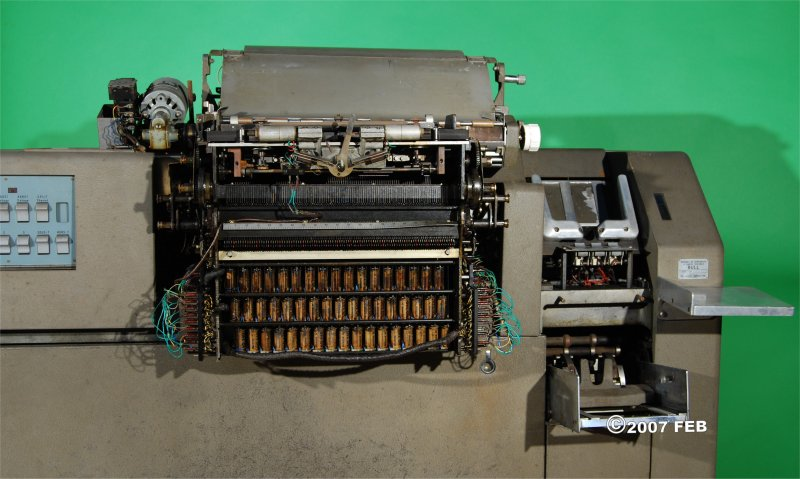
\includegraphics[scale=0.1]{tabulatrice_bs120.jpg}
		\caption{Tabulatrice BS120}
		\end{wrapfigure}
		conception de la tabulatrice BS120 à cycles indépendants qui sera l'un des facteurs 
		principaux de l'expansion de Bull pendant vingt ans.
		\paragraph{}
		partir de \begin{bf}1947\end{bf}, l'activité exportatrice, interrompue par la guerre, reprend vigoureusement. 
		Pendant les quinze années suivantes, le réseau international de Bull, va prendre une extension considérable et 
		constituer une des grandes forces de la compagnie. Ainsi, en Belgique, SOMECA, \begin{bf}qui représentait Bull AG en 
		1930 devient en 1942\end{bf}, la Société belge des machines Bull. En Suisse, la société Endrich A.G. partenaire de 
		Bull depuis 1930, devient en 1947 une filiale sous le nom de Bull Lochkartenmaschinen A.G. En 1949, se conclut une 
		association avec Olivetti pour créer une filiale de distribution en Italie : la société Olivetti-Bull. Dans les années 
		quarante, Bull est implanté en Hollande, en Allemagne et en Amérique du Sud.
		\paragraph{}
		\begin{bf}1948\end{bf}: Bull dépasse IBM sur le marché français avec 385 équipements installés. En seize ans, 
		le nombre d’équipements installés sera multiplié par dix. Il s'agit d'une croissance essentiellement interne, due au 
		développement des produits et des ventes. S'y ajoute l'absorption de certains sous-traitants de la compagnie. Cette 
		période est à la fois celle où le marché de la mécanographie atteint son apogée, et celle pendant laquelle Bull, de 
		même que ses concurrents, se convertit progressivement à l'électronique.
		\newline{}
		\paragraph{}
		\begin{bf}1951\end{bf}: \begin{bf}début de l’aventure informatique encore plus audacieuse\end{bf}. Bull présente, 
		\begin{wrapfigure}[13]{l}{4.5cm}
		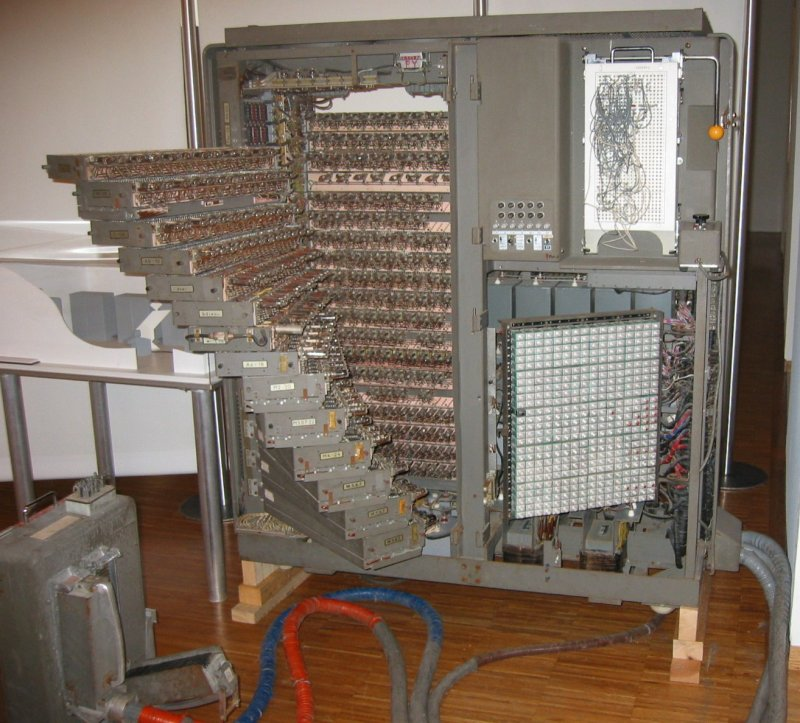
\includegraphics[scale=0.15]{gamma3.jpg}
		\caption{Gamma 3}
		\end{wrapfigure}
		à Paris, au 3ème SICOB (Salon des Industries et du Commerce de Bureau) le Gamma 3, son premier calculateur électronique, 
		relié aux machines de lecture et d’impression, il permet d’effectuer les calculs beaucoup plus rapidement. 
		Succès technique et commercial, le Gamma 3 devient un modèle de référence et annonce le déclin de la mécanographie et 
		le début de l’ère de l’informatique. Son programme, un simple enchaînement d’opérations, est câblé manuellement à 
		l’aide de petites fiches électriques que l’on insère en séquence dans des trous numérotés donnant accès aux fonctions 
		élémentaires de la machine. Il sera suivi par le Gamma 3 B à « tambour magnétique » utilisé aussi bien pour la gestion 
		que pour le calcul scientifique ; le tambour contient des programmes et des données intermédiaires. C'est une unité de 
		calcul rapide qui effectue des opérations comptables et scientifiques pour le compte d'une machine à cartes perforées 
		(tabulatrice BS 120) à laquelle il est connecté. Effectuant \begin{bf}5 800 opérations par seconde\end{bf}, 
		il exécute les calculs dans l’intervalle de lecture de 2 cartes consécutives, laissant la machine fonctionner à sa 
		vitesse nominale de 150 cartes minutes. L'innovation technique réside dans l'utilisation intensive de diodes au 
		cristal de germanium (\begin{bf}une première technologique\end{bf}) : le Gamma 3 ne comporte plus que 400 tubes 
		électroniques au lieu de 1 500 dans les appareils similaires, ce qui entraîne une réduction des coûts de fabrication 
		et une fiabilité fortement améliorée.
		\paragraph{}
		\begin{bf}1952\end{bf}: l’entreprise compte 2200 salariés. En \begin{bf}1956\end{bf} le marché soviétique s'ouvre 
		aux produits de la CMB. En 1960, Bull entre sur le marché de la République Populaire de Chine.
		\paragraph{}
		\begin{bf}En 1957\end{bf} Bull développe le système de codage (\begin{bf}C\end{bf}aractères \begin{bf}M\end{bf}agnétiques 
		\begin{bf}C\end{bf}odés à \begin{bf}7\end{bf} bâtonnets) encore utilisé aujourd’hui dans le traitement des chèques 
		bancaires notamment.
		\paragraph{}
		\begin{bf}1960\end{bf}: Bull lance « un grand frère » du Gamma 3 avec le Gamma 60, \begin{bf}premier ordinateur 
		multitâche au monde\end{bf}, doté d’une structure logique en avance de dix ans (20 fois plus rapide que le Gamma 3 et 
		beaucoup plus puissant de par sa capacité multitâches). Les données sont initialement introduites à partir de cartes 
		\begin{wrapfigure}[9]{l}{5cm}
		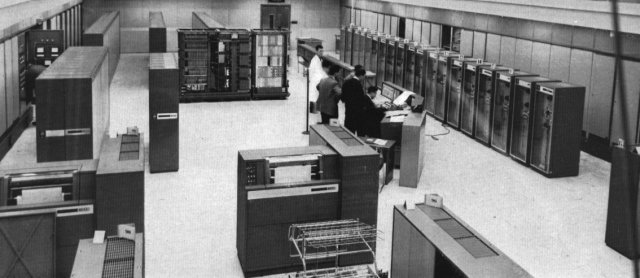
\includegraphics[scale=0.2]{gamma60.jpg}
		\caption{Gamma 60}
		\end{wrapfigure}
		perforées à 80 colonnes, à la vitesse de 300 cartes à la minute ; elles sont alors stockées sur rubans et tambours 
		magnétiques. Son développement conduit Bull à concevoir ses premiers éléments d’OS (Operating System). Il symbolise 
		l’apparition du monde des informaticiens avec ses grandes salles climatisées et ses nouveaux métiers : 
		les programmeurs, les analystes…. Il préfigure les grands systèmes qui s’imposeront pendant les trente années 
		suivantes et peut être considéré comme l’ancêtre du TERA 100. Une quinzaine de Gamma 60 seront vendus à des clients 
		prestigieux parmi lesquels on peut citer : SNCF, EDF, Mitsubishi Corp. et le CEA. \newline{}
		\newline{}
		Parallèlement Bull commercialisera le Gamma 10 conçu par Bull et véritable successeur du Gamma 3 et le Gamma 30 vendu 
		sous licence RCA comme le feront de leur coté Siemens et ICL. Le dernier Gamma 60 européen sera retiré du service en 
		1974.
		\newline{}
		\newline{}
		\newline{}
		\newline{}
		\paragraph{}
		\begin{bf}1962\end{bf}: lancement du Gamma 10, véritable successeur du Gamma 3 et dernier représentant de la 
		\begin{wrapfigure}[4]{l}{3.5cm}
		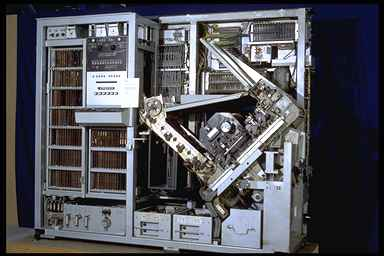
\includegraphics[scale=0.25]{gamma10.jpg}
		\caption{Gamma 10}
		\end{wrapfigure}
		génération « mécanographie à carte perforée » ; destiné aux applications de gestion, il utilise la technologie des 
		grands systèmes (ordinateurs de 2ème génération). En octobre \begin{bf}1962\end{bf} est signé un accord commercial 
		avec Mitsubishi qui reçoit l'exclusivité de la vente du matériel Bull sur le marché japonais et acquiert  un Gamma 60 
		puis des Gamma 10.
		\newline{}
		\newline{}
		\newline{}
		\newline{}
		\subsubsection{1962-1982: Alliances internationale}
		\paragraph{}
		\begin{bf}1962\end{bf}: La CMB atteint le 17ème rang des sociétés françaises cotées en bourse. Elle doit cette 
		performance à deux atouts majeurs : une gamme de produits adaptée aux besoins de la clientèle (dans les domaines de la 
		comptabilité-gestion et du calcul scientifique) ; et la mise en place de services efficaces de formation, d’assistance 
		technique et d’entretien. Ces prestations étaient le plus souvent intégrées dans le prix de location des machines, 
		lesquelles n’étaient que très rarement vendues.
		\paragraph{}
		\begin{bf}1963\end{bf}: fin 1963, la compagnie est présente dans 46 pays et exporte 60\% de sa production. Elle 
		occupe le deuxième rang mondial et le premier rang européen des industriels du traitement de l’information. \begin{bf}Bull 
		détient 1/3 du marché français, 10\% du marché européen\end{bf}.
		\paragraph{}
		\begin{bf}1964\end{bf}: La Compagnie des Machines Bull compte 15 600 salariés et réalise 60\% de son chiffre 
		d’affaires à l’exportation au travers d’un réseau de 22 filiales et agences servant 46 pays. C’est le \begin{bf}premier 
		constructeur européen et le deuxième mondial\end{bf}. Ce développement rapide nécessite des investissements importants 
		tant pour le financement des locations que pour celui des études de nouveaux produits et technologies : passage à 
		l’électronique, logiciels, élargissement de la gamme, etc…\newline{}
		En juillet 1964, le gouvernement autorise la prise de contrôle par le groupe américain General Electric, et la 
		compagnie prend le nom de Bull General Electric, avec pour mission, au sein du nouvel ensemble, de concevoir et 
		fabriquer les ordinateurs moyens et des périphériques.\newline{}
		L’histoire de Bull s’écrit désormais aussi de l’autre côté de l’Atlantique. L’apport de General Electric est 
		déterminant sur le plan de la gestion financière, du management, de l’organisation et des équipes d’études et de la 
		stratégie commerciale. GE apporte notamment son savoir faire en haut de gamme et plus particulièrement dans les 
		multiprocesseurs utilisés pour des applications critiques, prenant ainsi le relais du Gamma 60 dans le catalogue. 
		C’est à partir de cette année que sont distribués les ordinateurs de General Electric et CMB. \begin{bf}En juillet 1969, deux 
		ordinateurs Bull-GE assurent le contrôle des organes vitaux de la fusée Saturne qui emmène les astronautes d’Apollo XI 
		faire leurs premiers pas sur la lune\end{bf}. En France, le lancement en 1966 du Plan Calcul, prise de conscience de l’enjeu 
		de la souveraineté informatique, aboutira à la création de la CII (Compagnie internationale informatique). En 1967, 
		General Electric porte sa participation à 66\%.
		\paragraph{}
		\begin{bf}1970\end{bf}: Bull General Electric, dont les actionnaires sont la Compagnie des Machines Bull devenue 
		société holding, et General Electric. Mais en 1970 General Electric décide de ne pas poursuivre son activité 
		Informatique et cède celle-ci à un autre américain, Honeywell. Bull GE devient Honeywell-Bull.
		\newline{}
		\newline{}
		\paragraph{}
		\begin{bf}1973\end{bf}: lancement du Micral N, le premier microordinateur commercialisé au monde par la société R2E
		\begin{wrapfigure}[4]{l}{3cm}
		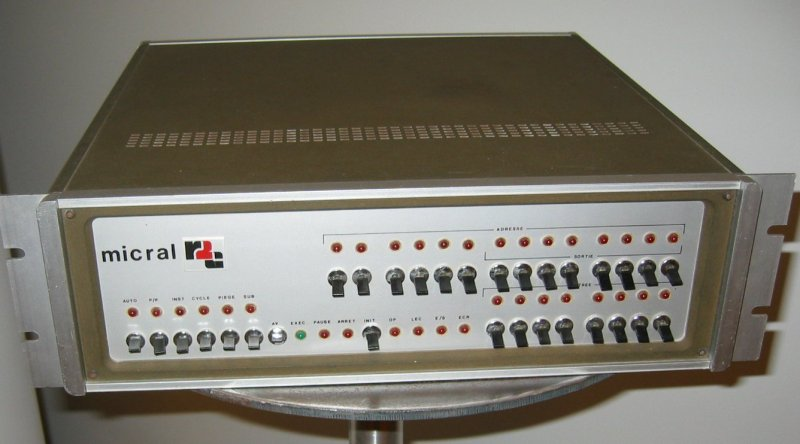
\includegraphics[scale=0.1]{micral_n.jpg}
		\caption{Micral N}
		\end{wrapfigure} 
		qui sera rapidement rachetée par Bull. Développé à partir d’un microprocesseur du commerce, Intel 8008, il préfigure 
		l’arrivée de l’informatique aussi bien dans les petites entreprises que chez les particuliers. Il marque aussi le 
		début d’une collaboration avec Intel qui deviendra très régulière.
		\newline{}
		\newline{}
		\newline{}
		\paragraph{}
		\begin{bf}1974\end{bf}: Honeywell-Bull, a structuré une gamme complète, la série 60, allant du mini-ordinateur aux 
		\begin{wrapfigure}[10]{l}{3.5cm}
		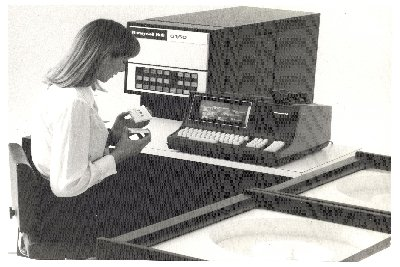
\includegraphics[scale=1]{serie_60.jpg}
		\caption{Serie 60}
		\end{wrapfigure} 
		grands systèmes et pour laquelle ont été développés les systèmes d’exploitation GCOS. Les produits sont conçus et 
		fabriqués tant aux Etats-Unis (PHOENIX le 66 et Boston le Mini 6), qu’en Europe (Pregnana le 62 et Paris le 61 et le 
		64 dont NEC acquiert la licence et en dérivera sa gamme de référence). Si ces produits sont des réussites, il n’en est 
		pas moins vrai que la multiplicité des laboratoires d’études freine la mise en commun de nombreux développements et 
		induit des coûts supplémentaires. Les produits équipent aussi bien les plus grandes organisations que des PME et tout 
		particulièrement dans ce cas, les applicatifs prennent une part déterminante dans l’atteinte des objectifs des clients.\newline{}
		La campagne de communication intitulée « L’informatique créative » reflète cette inflexion : Bull fait parler ses 
		clients : les marques Charles Jourdan, Knoll, Seb ou les restaurants Jacques Borel accepteront ainsi de témoigner de 
		leurs choix en faveur de Bull. Les partenariats avec les producteurs d’applicatifs que sont les SSII prennent une 
		ampleur déterminante et consommatrice de financement.
		\paragraph{}
		\begin{bf}1976\end{bf}: le gouvernement décide de regrouper Honeywell Bull avec les activités de la Compagnie 
		Internationale pour l’Informatique (CII, qu’il avait créée en 1966). Elle \begin{bf}choisit l’arbre comme symbole 
		fédérateur\end{bf}. L’arbre est un symbole universel de savoir, de croissance et de vitalité. Il représente l’avenir 
		et la croissance de Bull et de ses clients.\newline{}
		\begin{wrapfigure}[10]{l}{3.5cm}
		
\includegraphics[scale=0.25]{dsa_vf.jpg}
		\caption{DSA}
		\end{wrapfigure} 
		L’actionnaire majoritaire de la nouvelle compagnie CII Honeywell Bull redevient français (la CMB avec 53\% du capital). 
		En quatre ans, le chiffre d’affaires double mais le problème de financement de la croissance n’est pas résolu et 
		l’entreprise souffre de sous-capitalisation. En matière de coûts d’études, ce sont deux nouvelles lignes de produit à 
		faire converger avec les quatre précédemment citées ; un ambitieux programme est mis en place en ce sens dont la 
		réalisation la plus significative sera l’architecture de réseau DSA.
		\newline{}
		\newline{}
		\newline{}
		\newline{}
		\newline{}
		\newline{}
		\paragraph{}
		\begin{bf}1979\end{bf}: Saint-Gobain entre dans le capital de CMB et en devient majoritaire l’année suivante. Pour 
		accélérer les progrès technologique, CII Honeywell Bull crée un « Centre de Recherche » et intensifie ses coopérations 
		avec les milieux universitaires français et étrangers.\newline{}
		\begin{wrapfigure}[7]{l}{3.5cm}
		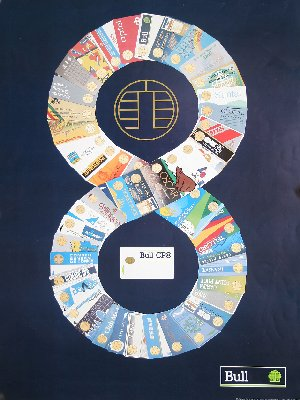
\includegraphics[scale=0.25]{cp8_affiche_vf.jpg}
		\caption{CP8}
		\end{wrapfigure}
		Cette année-là commence la commercialisation de la Carte CP8, « première à carte micro-processeur » ; cette « carte à 
		puce » (à distinguer de la simple carte à mémoire type paiement téléphonique) est destinée aussi bien à des 
		applications monétiques, qu’au contrôle d’accès ou à des dossiers portables. En plus de cette carte, Bull va proposer 
		progressivement des solutions complètes en maîtrisant également les terminaux de paiement ou les systèmes de 
		transactions sécurisés. Cette activité florissante sera finalement cédée vingt ans plus tard.
		\newline{}
		\newline{}
		\newline{}
		\newline{}
		\newline{}
		\paragraph{}
		Toujours en \begin{bf}1979\end{bf} CII Honeywell Bull annonce DSA (Distributed Systems Architecture), son 
		architecture de réseau. Alors que s’ouvre l’ère des réseaux d’ordinateurs, DSA était un ensemble de conventions et de 
		protocoles assurant la mise en connexion des systèmes et terminaux au travers de réseaux de transmission publics ou 
		privés. En permettant aux machines Bull de commencer à échanger leurs données depuis les quatre coins du monde, DSA 
		était symbolique du début du rapprochement entre l’univers des télécommunications et celui de l’informatique. Basée 
		sur des protocoles normalisés par l’ISO cette architecture, dans son approche, préludait au monde des « Open 
		architectures ». Une compétence que Bull a beaucoup développée depuis.\newline{}
		En \begin{bf}mai 1981\end{bf}, ce sont les équipes de Bull qui assurent, à la télévision, les \begin{bf}estimations 
		du résultat de l’élection présidentielle\end{bf}. Elles affichent pour la première fois, en direct, le visage numérisé du 
		vainqueur : François Mitterrand.
		\subsubsection{1982-1990: Dimension mondiale}
		\paragraph{}
		\begin{bf}1982\end{bf}: l’État devient l’actionnaire principal de la Compagnie des Machines Bull. Pôle de 
		développement de l’industrie informatique française, la compagnie voit sa compétence dans la mini-informatique 
		renforcée par l’annonce du regroupement de CII Honeywell Bull, de la SEMS (filiale du groupe Thomson), de DAP 
		(département des activités péri-informatique de Thomson) et de Transac (société d’informatique et de bureautique du 
		groupe Alcatel). La constitution d’un nouveau groupe autour de CMB a permis le redressement et le développement de CII 
		Honeywell Bull.\newline{}
		Cette même année, une nouvelle équipe menée par Jacques Stern et Francis Lorentz met en œuvre une politique de 
		croissance externe et d’investissement important dans la R\&D, l’outil industriel, la qualité et la force commerciale.
		\paragraph{}
		\begin{bf}1983\end{bf}: \begin{bf}choix du nom Bull\end{bf}. Cinquante années d’efforts et de progrès ont permis à 
		l’entreprise de conclure les alliances nécessaires, sauvegarder ses compétences, s’enrichir d’expérience multiples et 
		conserver intacte la volonté de développer une informatique européenne capable de s’imposer sur les marchés mondiaux.
		\paragraph{}
		\begin{bf}1984\end{bf}: François Mitterrand, Président de la République, vient chez Bull, le 2 mai 1984 célébrer la 
		sortie du 1000ème DPS7. Cet ordinateur de la gamme DPS qui a, depuis 5 ans, remplacé le modèle 64 de la série 60 
		rencontre un très grand succès commercial. Bull redevenue française en 1976, est désormais le leader européen de 
		l’informatique et de la bureautique, et met en œuvre en \begin{bf}1985\end{bf} une stratégie sur trois axes :
		\begin{itemize}
			\item Offre à l’usager d’informatique distribuée (poste de travail, serveurs départementaux, accès aux systèmes 
			informatiques)
			\item Offre solution (approche sectorielle avec les SSII, ouverture au monde informatique, services associés)
			\item Coopération technologique et prospective (programmes de recherche européens, accords mondiaux sur produits 
			à haute technologie)
		\end{itemize}
		\paragraph{}
		Au début des années 80, Bull cherche une idée novatrice pour dynamiser son image de marque et son personnel. 
		Elle décide de sponsoriser un projet, à l'époque très audacieux : \begin{bf}financer un voilier de course pour gagner 
		la WHITBREAD\end{bf}, la course à la voile la plus prestigieuse du moment. L'idée est de créer un état d'esprit au 
		sein d'une équipe soudée. C'est ainsi que les voiliers de course furent appelés \begin{bf}ESPRIT D'EQUIPES\end{bf}. 
		C'est LIONEL PEAN qui eut la responsabilité d'amener ce projet à terme. Il remporta la WHITBREAD le 12 mai 1986, ce 
		fut le premier voilier français à gagner cette course.
		\paragraph{}
		\begin{bf}En 1988\end{bf} Bull sort un système DPS7 en technologie CMOS deux ans avant ses concurrents ; en 
		\begin{bf}1991\end{bf} le chip du haut de gamme de cette ligne est plus dense que celui réalisé par Intel pour ses 
		propres processeurs ; il faudra attendre Itanium pour être dépassé par les chips des grands fondeurs. Mais les volumes 
		ne suivent pas, souvent faute d’offre applicative laquelle se focalise progressivement sur les architectures IBM et 
		Unix ; mais aussi le volume de vente des PC fournit aux fournisseurs de leurs CPU une assise incomparable pour 
		financer les générations successives.
		\paragraph{}
		\begin{bf}1987\end{bf}: à la suite de la décision de Honeywell de se retirer de l’informatique, Bull reprend les 
		activités de son partenaire américain Honeywell Information Systems, exercées dans une nouvelle société, Honeywell 
		Bull Inc. dont le siège est à Minneapolis. Bull (42,5\%) Honeywell (42,5\%) et NEC (15\%) s'en partagent le capital, 
		et en prend le contrôle en \begin{bf}1988\end{bf} ; tout comme Zenith Data Systems, constructeur américain de 
		micro-ordinateurs, en \begin{bf}1989\end{bf}. Parallèlement à ces acquisitions, Bull s’appuie sur une politique de 
		coopération intensive avec de nombreuses entreprises et institutions publiques et privées (aux échelles européenne et 
		mondiale) en matière de produits, procédés ou pour l’élaboration de standards internationaux.\newline{}
		Dans ces années-là, Bull et Honeywell se retireront progressivement de la fabrication de périphériques disques puis 
		bandes et enfin imprimantes, ces composants standardisés étant désormais achetés auprès de fournisseurs spécialisés 
		qui, petit à petit, fourniront toute l’industrie y compris IBM. Bull Belfort ferme en 1991.
		\paragraph{}
		\begin{bf}1990\end{bf}: coopération avec le groupe Videoton pour l’implantation de Bull en Hongrie et dans les pays 
		de l’Est. Des coopérations similaires sont initialisées en Inde et au Brésil, sans générer d’inflexion significative 
		des revenus. 
		\subsubsection{1991-1997: Actionnariat, privatisation, intense adaptation de l’offre et de l’organisation}
		\paragraph{}
		\begin{bf}1991\end{bf}: ouverture du capital de CMB à France Télécom et NEC.\newline{}
		En 1991, Bull commence à revoir à la baisse les ambitions de la stratégie d'expansion. Le marché des systèmes GCOS 
		commence en effet à s'éroder, en raison des coûts de développement encore élevés et de la limitation de l'effort 
		commercial au parc existant.\newline{}
		Les systèmes ouverts se montrent décevants, la clientèle n'ayant plus ou presque de raison à rester fidèle au même 
		fournisseur. Une tentative pour retrouver une économie de "mainframe" sur une base de système ouvert est tentée avec 
		le programme Sagister, qui reste bien en deçà de ses espoirs.\newline{}
		Bull entreprend de s'allier avec un partenaire informatique pour une collaboration sur les systèmes UNIX. Après une 
		investigation tous azimuts (incluant Intel, Digital Equipement et des plus petites sociétés), la recherche se porte 
		sur IBM qui avait plus de raisons de respecter l'indépendance de Bull.
		\paragraph{}
		\begin{bf}1992\end{bf}: Pour sa gamme UNIX, Bull doit sélectionner une architecture offrant les meilleurs potentiels 
		en matière d’évolutivité et de partenariats. Bull adopte l'architecture PowerPC (commune à IBM et à Motorola) : un 
		multiprocesseur destiné à être vendu par IBM et Bull, et fait l’objet d’une coopération technique dans le domaine du 
		logiciel (Grenoble). Dans le cadre de cet accord, IBM prend 4,5\% du capital de Bull.
		\paragraph{}
		\begin{bf}1994\end{bf}: recapitalisation par l’Etat français et France Télécom, avec pour mission un redressement 
		viable permettant une future privatisation.
		\paragraph{}
		\begin{bf}1995\end{bf}: L’Etat réduit sa part chez Bull grâce à une ouverture du capital et à la constitution d’un 
		socle d’actionnaires industriels durables, cohérent avec le développement du groupe et de ses métiers. Entrée de 
		Motorola (17\%), Dai Nippon Printing (DNP, 3,3\%) et du personnel de Bull (4\%). L’Etat conserve 37\% (79,6\% 
		précédemment).
		\paragraph{}
		\begin{bf}1997\end{bf}: la part du secteur public (Etat français 30,5\% et France Télécom 18,5\%) passe en février 
		sous la barre des 50\%, laissant la majorité aux actionnaires privés, aux industriels et aux salariés. Cette stratégie 
		permet à Bull de concentrer ses efforts dans les secteurs à forte valeur ajoutée où sa compétence est reconnue et 
		recherchée, et de s’appuyer sur ses partenaires industriels pour offrir des solutions globales à ses clients.\newline{}
		La privatisation s’achève avec l’ouverture du capital au public, réalisée en avril. Cette étape fait passer la part de 
		l’Etat à 17,3\%, France Télécom, Motorola et NEC portent leur participation à 17,7\%, DNP à 5,5\% et le flottant 
		(institutionnels, individuels et salariés) à 24\%.\newline{}
		Nomination en septembre de Guy de Panafieu à la présidence du Groupe. Maintenir les métiers traditionnels les plus 
		rentables et développer les futurs métiers de croissance sont les priorités, exprimées dans le Plan Stratégique 2002. 
		Bull décide de concentrer ses efforts dans les logiciels de sécurité, l’administration de systèmes et de réseaux, 
		la carte à microcalculateurs et le commerce électronique.\newline{}
		Bull développe également ses compétences dans les services, dans les activités d’intégration de systèmes, 
		d’infogérance, l’informatique en réseau, internet et intranet, secteurs en pleine croissance. Mais le coût de ces 
		adaptations quelque peu tardives dépasse les capacités d’autofinancement sans pour autant atteindre la masse critique 
		permettant d’être profitable. \newline{}
		\paragraph{}
		Du point de vue de l'offre, les ambitions d'être un acteur de l'industrie du logiciel sont considérablement réduites 
		\begin{wrapfigure}[11]{l}{5.5cm}
		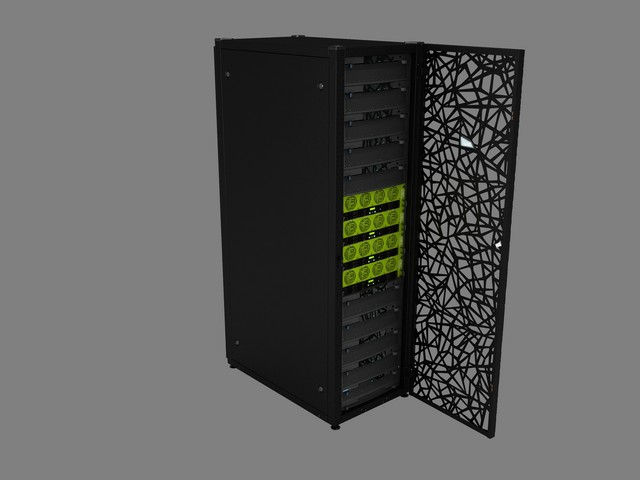
\includegraphics[scale=1]{novascale.jpg}
		\caption{Novascale}
		\end{wrapfigure} 
		et progressivement, Bull reconnait que Linux (comme système d'exploitation) et Internet (dans les réseaux) s'avèrent 
		incontournables. De même, dans le domaine des processeurs, Bull renonce progressivement à développer son offre PowerPC 
		pour se tourner vers Intel.\newline{}
		En bas de gamme, son alliance avec NEC lui permet de commercialiser des machines x86. En haut de gamme, Bull prépare 
		des machines Itanium pour lesquelles il développe ce qui est aujourd'hui connu comme la gamme NovaScale.\newline{}
		Pour cette gamme de produits, Bull a développé des émulateurs de ses systèmes GCOS de façon à ne plus avoir à 
		supporter des dépenses de hardware pour les deux lignes de produits propriétaires subsistantes.\newline{}
		\newline{}
		\newline{}
		\newline{}
		La gamme NovaScale a permis en outre à Bull de prendre une position unique en Europe dans le domaine très compétitif 
		des superordinateurs (Tera 10).
		\paragraph{}
		Tout ceci implique que Bull apprenne de nouveaux métiers et tisse de nouvelles alliances sans pouvoir laisser de coté 
		certains métiers traditionnels. C’est dans cette période que les études de Bull redéployent sur des processeurs 
		standards Intel les architectures DPS de milieu et haut de gamme. Toujours dans cette période, les études réalisent 
		les premiers clusters de multiprocesseurs (jusqu’à 16 processeurs) à la base des interconnexions des HPC d’aujourd’hui, 
		et créent les premières « practices » ciblant quelques métiers clients grâce à des accords avec les grands fournisseurs 
		de progiciels. 
		\subsection{Aujourd'hui}
		\subsubsection{Cap sur l'innovation}
		\paragraph{}
		Depuis le début des années 1990, le Groupe a connu plusieurs restructurations, dont la dernière s'est achevée en 2004 
		sous l’impulsion du président Pierre Bonelli. (recapitalisation de 400 millions de francs avec l'aide de l'État français).
		\paragraph{}
		\begin{bf}Début 1999\end{bf}, les effectifs de Bull étaient légèrement supérieurs à 20 000 personnes. Fin 2001, 
		les effectifs de la société s’élèvent à 10 000 personnes.
		\paragraph{}
		\begin{bf}2000\end{bf} : Depuis toujours soucieux d’apporter à ses clients les moyens de profiter des opportunités 
		offertes par la technologie, Bull entend les aider à entrer dans la « nouvelle économie ». La campagne 
		« Network of confidence » illustre parfaitement la démarche proposée : faire évoluer les infrastructures et transformer 
		les processus pour s’intégrer au réseau et tirer parti de son potentiel, mais aussi mettre l’accent sur la sécurité. 
		Bull a déjà compris que la confiance serait l’un des piliers de la société numérique alors en gestation.
		\paragraph{}
		\begin{bf}2001\end{bf} : le Groupe vend son activité cartes à puce à Schlumberger, aujourd'hui Gemalto. Il vend 
		également des activités de services en Europe à Steria (hors France).
		En matière d’offre, Bull confirme un engagement technologique novateur dans les technologies ouvertes, qui conduit 
		\begin{bf}dès 2002\end{bf} à la fondation du premier consortium mondial dédié aux logiciels d’infrastructure libres, 
		ObjectWeb (aujourd’hui OW2), et au lancement en 2003 d’une nouvelle génération de serveurs ouverts pour les 
		applications commerciales et scientifiques, NovaScale.
		\paragraph{}
		\begin{bf}2004\end{bf} : Bull prend la commande d'un super-ordinateur de la part de la division simulation du CEA/DAM.
		\paragraph{}
		\begin{bf}2005\end{bf} : Sortant victorieux d’une période complexe de restructuration, le groupe Bull prend 
		conscience d’un déficit d’image et décide de reprendre la parole pour marquer son retour. Un nouveau logo, un slogan 
		« Architecte d’un monde ouvert » qui définit son périmètre et la restructuration progressive de son offre autour de 
		produits et solutions innovantes : NovaScale, globull, mobull, bullx, bullion, biodatacenter … viennent renforcer sa 
		position de leader européen des systèmes numériques critiques.
		Une offre de services globale est lancée, permettant de concevoir, bâtir et exploiter les applications critiques 
		d’entreprise en s’appuyant sur toute la richesse fonctionnelle des logiciels libres. La signature de contrats 
		d’envergure mondiale confirme le succès de cette stratégie ainsi que le potentiel technologique et commercial du Groupe.
		\newline
		En \begin{bf}Mars\end{bf}, le gouvernement vend le reste de sa participation dans Bull. France Télécom reste 
		l'actionnaire le plus important.
		\paragraph{}
		\begin{bf}Novembre 2005\end{bf} : livraison du Tera 10, super-ordinateur au CE/DAM. Tera 10 forme un cluster de 
		544 noeuds de calcul NovaScale, comportant chacun huit processeurs double cœur Intel® Itanium® 2 de nouvelle 
		génération. L'ensemble constitue une capacité de traitement de 4532 processeurs double cœur et 30 Tera octets de 
		mémoire centrale. La performance atteinte, mesurée sur 4000 processeurs, est de 42,9 Tera flops, démontrant ainsi la 
		remarquable efficacité de l’infrastructure retenue pour Tera 10.
		\paragraph{}
		\begin{bf}L’année 2006\end{bf} a été une année de transformation du Groupe, associant d’importantes avancées, 
		notamment dans le calcul haute performance, les télécommunications et les services.
		La transformation du Groupe s’est poursuivie en 2007 avec des acquisitions ciblées – en particulier l’acquisition 
		en Espagne de la société de services Siconet, et en France celle de Serviware, principal intégrateur de solutions pour 
		le Calcul haute performance.
		\paragraph{}
		\begin{bf}En 2007\end{bf}, Bull lance son programme 7i. Ce sont sept initiatives pour aider les entreprises à 
		tirer profit d’un monde ouvert. Conjuguant le meilleur des services et des technologies ouvertes, Bull entend aider 
		les entreprises à faire de leurs systèmes d’information (SI) un levier de création de valeur dans un monde connecté, 
		en facilitant croissance, compétitivité et souveraineté.
		\paragraph{}
		\begin{bf}L’année 2008\end{bf} a permis de poursuivre la voie de la transformation du Groupe et du développement de 
		ses activités d’avenir, avec en particulier l’acquisition en Belgique de CSB Consulting, société de services 
		informatiques, et en Allemagne de la société science+computing, leader dans les services et les solutions pour le 
		Calcul haute performance.
		Bull emploie environ 7 800 salariés et recrute à nouveau fortement (1000 personnes en 2008), ce qui porte le total des 
		salariés à 8 850 en 2009.
		\paragraph{}
		\begin{bf}En 2009\end{bf} Bull confirme sa position d’acteur européen majeur de l’économie numérique avec le 
		lancement d’innovations significatives : bullx (élu meilleur supercalculateur au monde), mobull 
		(une révolution des centres de données), et des réalisations de très grande envergure (Chorus, supercalculateur pour le 
		Forschungszentrum Jülich en Allemagne, hébergement et exploitation de mon.service-public.fr, etc.). Le chiffre 
		d'affaires est de 1,1 milliard d'euros en 2009, réalisé à 52\% en France.
		\paragraph{}
		\begin{bf}L’année 2010\end{bf} a permis à Bull de prendre une nouvelle dimension, avec le lancement de nouveautés 
		importantes (notamment la refonte de ses gammes de serveurs pour le calcul haute performance, les grands systèmes 
		Windows/Linux et les mainframes), des réalisations de très grande envergure (livraison de Tera 100, premier 
		supercalculateur européen), lancement d’une offre innovante pour le calcul à la demande (extreme factory) et 
		l’acquisition du groupe Amesys, un leader européen dans la sécurité et les systèmes critiques.
		\paragraph{}
		\begin{bf}Novembre 2010\end{bf} : le \begin{bf}supercalculateur Tera-100 du CEA se classe à la 6ème place mondiale\end{bf} 
		avec 1,05 pétaflops sur Linpack et 1,25 en puissance crête théorique. C'est le tout premier calculateur européen à 
		\begin{wrapfigure}[7]{l}{3.5cm}
		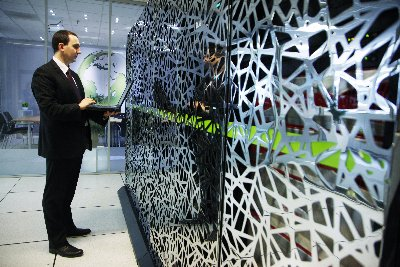
\includegraphics{tera_100.jpg}
		\end{wrapfigure}
		passer la barre symbolique du pétaflops et il est constitué de 4 370 serveurs bullx pour un total de 17 480 processeurs 
		octo-cœurs Intel Xeon 7500 (près de 140 000 cœurs en tout). Le chiffre d’affaires est de 1,25 milliard d’euros, 
		réalisé à 56,3\% en France. Le Groupe est présent dans 50 pays, sur tous les continents, et emploie 8750 collaborateurs.

		Le plan stratégique BullWay 2011-2013, annoncé \begin{bf}fin 2010\end{bf} par son nouveau PDG Philippe Vannier, a 
		pour objectif de positionner Bull sous trois ans comme un leader européen des systèmes numériques critiques et de 
		mettre le Groupe sur le chemin d’une croissance rentable.
		\subsection{Organisations}
			Bull est organisé en quatre grande partie appelées Bussiness Lines
			\subsubsection{Security Solutions}
			\subsubsection{Business Integration Solutions}
			\subsubsection{Computing Solutions}
			\subsubsection{Innovative products}
	\section{Le secteur d'activité}
		\subsection{Présentation}
			les concurrents, les besoins des consommateurs...
			Quatre secteurs de prédilections
			\subsubsection{Secteur public}
			\subsubsection{Finace}
			\subsubsection{Défense}
			\subsubsection{Télécom}
		\subsection{Actualités}


\newpage
\rhead{Le cadre du stage}
\part{Le cadre du stage}
	\section{Description de la structure sociale}
		La société [•] regroupe [ effectif / nombre ] d’employés (on compte environ [•] employés au sein de la société [•] 
		dans le monde), qui sont divisés en [•] départements, tous sous la direction du Président-directeur général, [•]: 
		Equipe performance secteur R\&D (5 membres)
		Organigramme à présenter.
	\section{Fonctionnement}
		Au sein de cette société de taille [•], il est aisé de percevoir l’interaction constante entre les différents 
		services décrits plus haut. On distingue [•] circuits de création de richesse suivant qu’il procède [•] ou de [•].
		Compte tenu du fait que mon stage a été exclusivement réalisé au service de [•] ,et que [•], il sera uniquement 
		développé le [•].
		[Description du processus dans lequel on travaille. Plusieurs page d’explications et éventuellement de définitions].

\newpage
\rhead{Travaux effectués et apports du stage}
\part{Travaux effectués et apports du stage}
		La mission principale du stage a consisté à étudier l'accélerateur d'Intel. Le but étant d'évaluer les performances de la carte,
		mais aussi d'en comprendre le fonctionnement tant sur le plan matériel que logiciel. La carte présente dans nos bureaux,
		appelé Knights Ferry était une version alpha. Une version beta (Knights Corner) fut disponible plus tard dans les bureaux
		d'Echiroles et je pu effectuer des tests sur cette carte également.
		J'ai également travailler sur le projet OpenGPU en partenariat notamment avec l'Ecole Centrale de Paris et le CEA,
		en faisant des tests comparatifs en GPU et CPU.
		Pour mener à bien ces missions différents matériels étaient à disposition.
		J'ai appris pas mal de choses l'autonomie, le travaille en groupe et surtout à trouver des solutions aux problèmes.
	\section{Travaux effectués}
		\subsection{Les outils}
			J'avais un ordinateur personnel avec le choix de l'environnement. J'y ai installé Ubuntu.\newline
			Un second ordinateur, qui contenait l'accélerateur Intel, était à disposition de toute l'équipe:\newline
				(Description de la machine)\newline
			Des serveurs étaient également disponible pour l'équipe avec du matériel varié:\newline
				(description des lames... tableaux ect...)\newline
			Finalement on eu accès au Knights Corner d'Echirolles:\newline
				(description machines echirolles)\newline
		\subsection{Les missions}
			\subsubsection{Knights Ferry}
				\paragraph{}
				Knights Ferry est le nom donné à la carte MIC (Many Integrated Cores) d'Intel dans sa version alpha. Il s'agit 
				d'un accélérateur assez similaire à un GPU dans le sens où l'on peut exécuter des noyaux de calcul sur la 
				carte afin d'accélerer les programmes. La mission principale était de comprendre le fonctionnement de cette
				carte, d'en évaluer dans un premier temps les performances théoriques puis dans un deuxième temps les 
				performances réelles sur des programmes de tests. Aussi, toutes les connaissances et touts les résultats ont 
				été systématiquement reportées sur un wiki interne.
				\paragraph{Documentation}
				Ce materiel étant nouveau et encore dans une version d'Alpha, son fonctionnement tant au niveau hardware que
				software était encore inconnu. Il aura donc fallu avant tout lire la documentation fournie. Ceci m'a permi de 
				connaître les propriétés hardware de la carte, comme le nombre de coeurs, de threads par coeur ou encore 
				la taille des registres. Ce travail a été indispensable pour estimer les performances théoriques de la carte 
				et pouvoir coroborer les performances observées avec le matériel. \newline
				J'ai également pu noter la procédure d'installation des drivers, et de manière générale l'utilisation
				de la carte à savoir comment démarrer le MIC, ou encore comment compiler un code pour la carte et les 
				différents modes d'exécution. \newline
				J'y ai également trouvé la liste des outils indispensables comme le debuggeur ou encore un programme de
				monitoring (voir figure 12) ainsi que plusieurs outils d'information et de configuration.
				\begin{figure}
				\begin{center}
				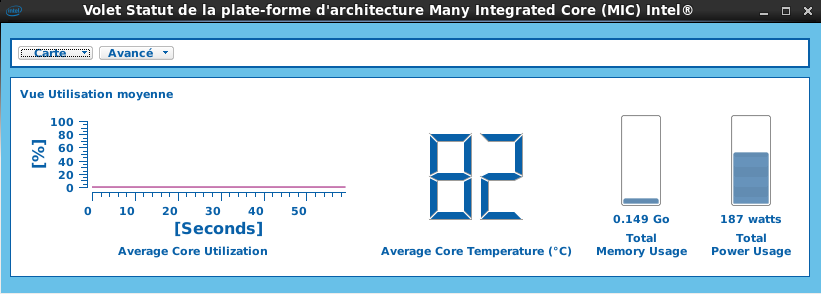
\includegraphics[scale=0.40]{monitor_mic.png}
				\caption{Monitoring MIC}
				\end{center}
				\end{figure}
				\paragraph{Drivers}
				La premiere chose à faire a donc était l'installation de la carte et des drivers puis de vérifier le bon
				fonctionement de la carte. Cette étape s'ai déroulé sans problème, en effet l'installation consistait en 
				l'exécution d'un simple script python, et les outils fourni m'ont permi de constater que la carte était
				correctement installée et reconnue.
				\paragraph{Benchmark pour le MIC}
				Dès lors, le but était de pouvoir évaluer les performances de l'accélerateur tels que le débit mémoire,
				la puissance de calcul, les latences etc.. \newline
				Il existe de nombreux programmes de benchmark disponibles, l'idée était donc de porter les tests en notre
				possession sur le MIC, ce qui dans un premier temps était peut-être moins adapté au hardware particulier
				de la carte, mais nous permettrait d'appéhender le matériel et d'obtenir des résultats plus rapidement 
				que s'il avait fallu écrire des tests spécifiques au MIC.
					\subparagraph{}
					L'équipe avait donc un ensemble de tests, écrit en C, pour annalyser les performances d'une machine sur 
					chacun de ses composants. Il m'a donc était demandé de porter ses tests pour le MIC. \newline
					Contrairement au GPU classique NVidia ou AMD, des codes en C ou FORTRAN existant peuvent directement
					s'exécuter sur le MIC si le bon flag a été donnée à la compilation. Ceci rend le portage de code
					simple et rapide. De cette manière le programme se lance, et s'exécute intégralement sur la carte
					sans interaction avec l'hôte.\newline
					La plus grosse difficulté a donc été de compiler correctement ces tests. Il aura fallu pour cela editer 
					les Makefile inclure les bon headers et correctement linker les différentes bibliothèques spécifiques au 
					MIC. (Rajouter qu'au départ, plusieurs bench ne se compilaient même pas, que d'autres se compiler, 
					mais ne se lancer pas sur le MIC, à cause de lib dynamique manquante, mais surtout du manque de 
					connaissance sur le fonctionnement de la carte. D'autres tests s'exécutaient, mais donnaient des résultats 
					plus que douteux. Finalement, certains se sont avéraient bien utils) \newline
					\subparagraph{}
					Parmi les programmes de tests standard qui permettent de classifier les différentes machines SpecINT et 
					SpecFP sont parmis les plus souvent utilisés. Il a donc semblé intéressant de les exécuter sur le MIC
					afin de pouvoir comparer la carte à d'autre solution de calcul. \newline
					CPU2000 est un ensemble de benchmark conçu pour tester les performances des CPU des serveurs. Le programme
					est écrit princpalement en perl, bash et C. Les tests en eux mêmes sont écrits en C et C++, et Il est 
					divisé en deux parties: CINT2000 et CFP2000 pour la partie flotante simple précision. \newline
					L'exécution de SPECInt peut se décomposer en quatre grandes étapes: \newline
					\begin{description}
					\item[Compilation :]
						Les différents programmes de test sont compilés, et les paramètres sont donnés à l'aide d'un fichier
						de configuration édité au préable pour la machine sur laquelle doit être exécuté SPECInt
					\item [Configuration :]
						Etant donné les tests à exécuter et les paramètres choisis (taille des données en entré, type de test
						à effectuer) les différents benchs sont paramétrés.
					\item [Exécution :]
						Les tests sont effectués, et sont mesurés grace à un binaire nomé "specinvoke".
					\item [Résultat :]
						Les résultats des tests sont compilés, et plusieurs fichiers de sortis sont créés (html, asc etc...)
						pour résumer les performances.
					\end{description}
					Il y avait alors deux possibilités pour utiliser SPECInt sur le MIC. Soit tout faire sur le MIC, soit 
					ne faire que la partie exécution et mesures sur la carte. \newline
					La deuxième solution a été rapidement choisie car la première avait de nombreux inconvénient. En effet il 
					aurait fallu recompiler l'ensemble de SPECInt pour MIC pour que les outils et binaire puisse s'exécuter
					dessus. Il aurait également fallu à chaque redémarage de la carte, réinstallé SPECInt dessus ou alors 
					créer une image du système pour le MIC avec SPECInt installé. Ces solutions étaient beaucoup trop complexes
					et le choix de la cross-compilation a donc été préféré. \newline
					Ainsi, s'il est précisé dans le fichier de configuration, que les tests sont destinés à un matériel de type
					MIC, alors la compilation se fera sur la machine hôte mais pour Knights Ferry. \newline
					La configuration se fait de la même manière quelque soit le support des tests. \newline
					L'exécution doit évidemment se faire sur la carte, l'ensemble des fichiers nécessaires aux tests en questions
					sont donc envoyés sur le MIC. A la fin de l'exécution, les fichiers de résultats sont rapatriés vers l'hôte. \newline
					Enfin les résultats sont analysés normalement.
					\subparagraph{}
					Une fois SPECInt fonctionnel pour MIC, l'interêt a donc été de le comparer à un processeur généraliste
					de type Sandy Bridge, mais surtout d'en analyser les résultats et d'en comprendre les raisons.
					(Expliquer la démarche de comparaison sans entrer dans les résultats)
					\subparagraph{}
					SPECOMP!
				\paragraph{Tests de performances}
				Pour étudier plus finement les performances il fallu écrire des tests moins généralistes et plus spécifiques
				à certaine partie de la carte, comme le processeur ou la mémoire.
					\subparagraph{}
					Les tests de calculs donnaient des résultats très inferieurs aux performances théoriques et performances 
					attendues. Après analyse il s'avera que les codes n'etaient que très rarement vectorisés du à un compilateur 
					en version alpha, que les bibliothèques de calculs étaient toujours en cours de dévelopement et donc pas 
					encore optimisées pour le MIC et que la seule façon d'obtenir les performances maximums seraient d'utiliser
					des instruction de type FMA (fused multiply-add) qui réalisent en une instruction des multiplications et 
					des additions sur un vecteur. \newline
					En partant d'un code assembleur qui permettait de vérifier qu'un processeur supportait l'AVX, nous avons 
					pour chacun des 32 registres de chaque processeur exécuter l'instruction \emph{vmadd213ps} qui réalise le 
					produit de deux vecteurs 512 bits (soit 16 floats) puis additionne tout les éléments du vecteur résultat.
					Une seule instruction réalise donc 32 opérations simple précision.
					Comme on exécute cette instruction pour les 32 registres, l'ensemble du code réalise 1024 opérations simple
					précision (Voir figure 13). Ainsi les pipelines des processeurs sont bien remplis et tout les registres sont
					utilisés. Ce code a permis d'atteindre 90.75\% de la performance crête théorique.
					\begin{figure}
					\begin{center}
					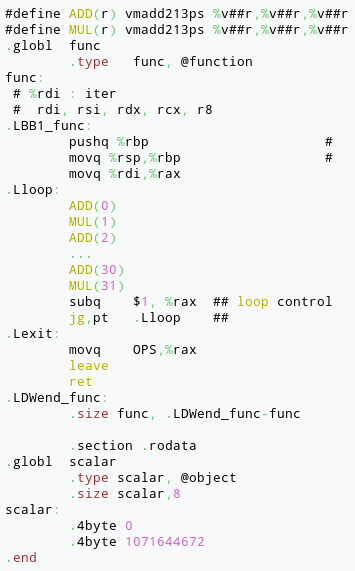
\includegraphics[scale=0.40]{assembleur.png}
					\caption{Assembleur}
					\end{center}
					\end{figure}
					\subparagraph{}
					Toujours pour tester la puissance de calcul de la carte, mais sur un test moins artificiel, nous avons voulu
					voir les performances pour des calculs matriciels. SGEMM et DGEMM (pour sa version double precision) sont 
					des fonctions de multiplications de matrices très bien implémentées et optimisées dans les bibliothèques de 
					calcul notemment dans la MKL (Maths Kernel Library) d'Intel. \newline
					La première implémentation du test s'exécutait sur la machine hôte, et seule la partie de calcul était 
					exécutée sur le MIC. Il était cependant difficil de pouvoir mesurer uniquement les temps de calculs. En effet
					l'implémentation pour le MIC de ce type de fonctionnement en sous-traitance, ne sépare pas clairement les 
					parties transfert de données vers la carte des parties de calcul. Il était donc difficil de mesurer uniquement 
					les calculs effectués sur le Knights Ferry. \newline
					La seconde version du test était donc complétement exécuté sur la carte. Pour pouvoir mieux visualiser
					les performances, j'ai implémenté une fonction d'affichage graphique dans le code afin d'avoir instantanément
					un résultat visuel (voir figure 14).
					\begin{figure}
					\begin{center}
					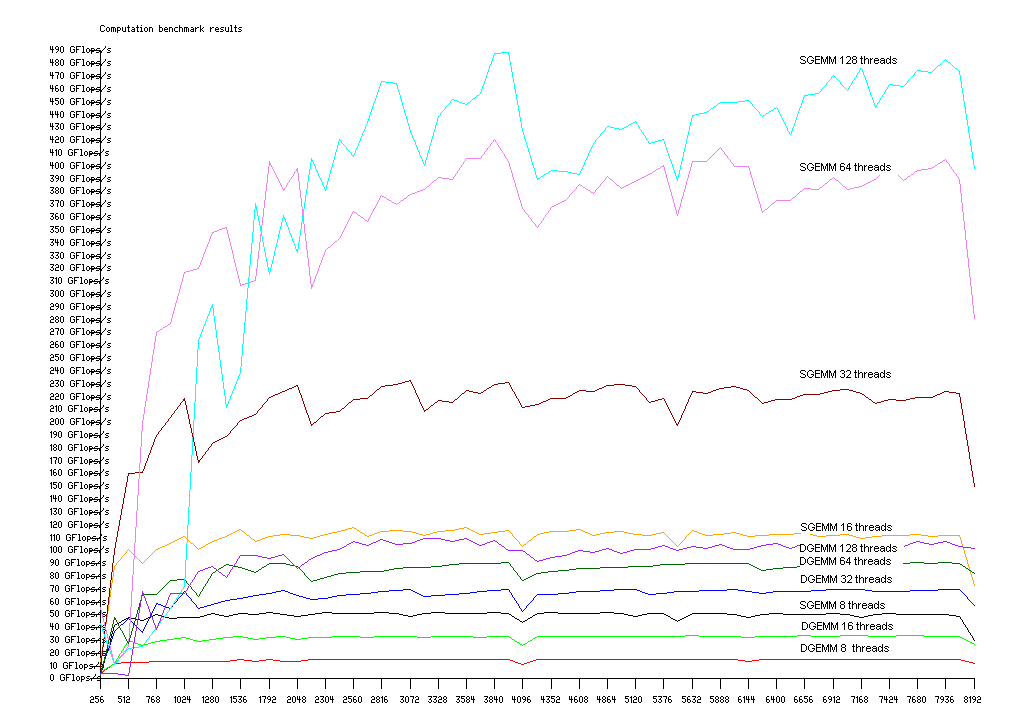
\includegraphics[scale=0.4]{gflops_SGEMM.png}
					\caption{Multiplication Matricielle}
					\end{center}
					\end{figure}
					\subparagraph{}
					Un autre composant important à tester est la mémoire. J'ai donc commencer le développement d'un test de mesure
					de débit. Je me suis pour cela inspiré d'un code existant et qui consisté à faire des chargements mémoires
					de données de taille croissante. Ainsi le débit de chaque niveau de mémoire pouvait être mesuré. Le code de base étant 
					écrit en assembleur, il a tout d'abord fallu le réecrire pour utiliser les instructions propres au MIC. 
					Malheureusement certaines instructions ne pouvaient pas être remplacées. En conservant les anciennes, le 
					matériel n'etait pas complétement exploité, et les débits mesurés étaient très loin de ceux espérés.
					J'ai donc réécrit le code en utilisant des intrinsics, et être ainsi sûr d'utiliser toutes les ressources
					de la carte. Mais encore une fois les débits n'étaient pas ceux annoncés. Après analyse, il paru évident
					qu'il n'était pas possible de saturer le débit mémoire en faisant travailler qu'un seul processeur.
					J'ai donc exécuté le même programme sur plusieurs coeurs jusqu'a arriver a une limite supérieur, qui 
					n'était plus très loin des débits théoriques (Voir figure 15). Cependant, contrairement aux tests sur 
					Ivy Bridge (voir figure 16), les débits du cache sont erronés. Sans doute à cause du trop grand nombre 
					de threads voulant accéder au cache, et qui sont donc pénalisés.
					\begin{figure}
					\begin{center}
					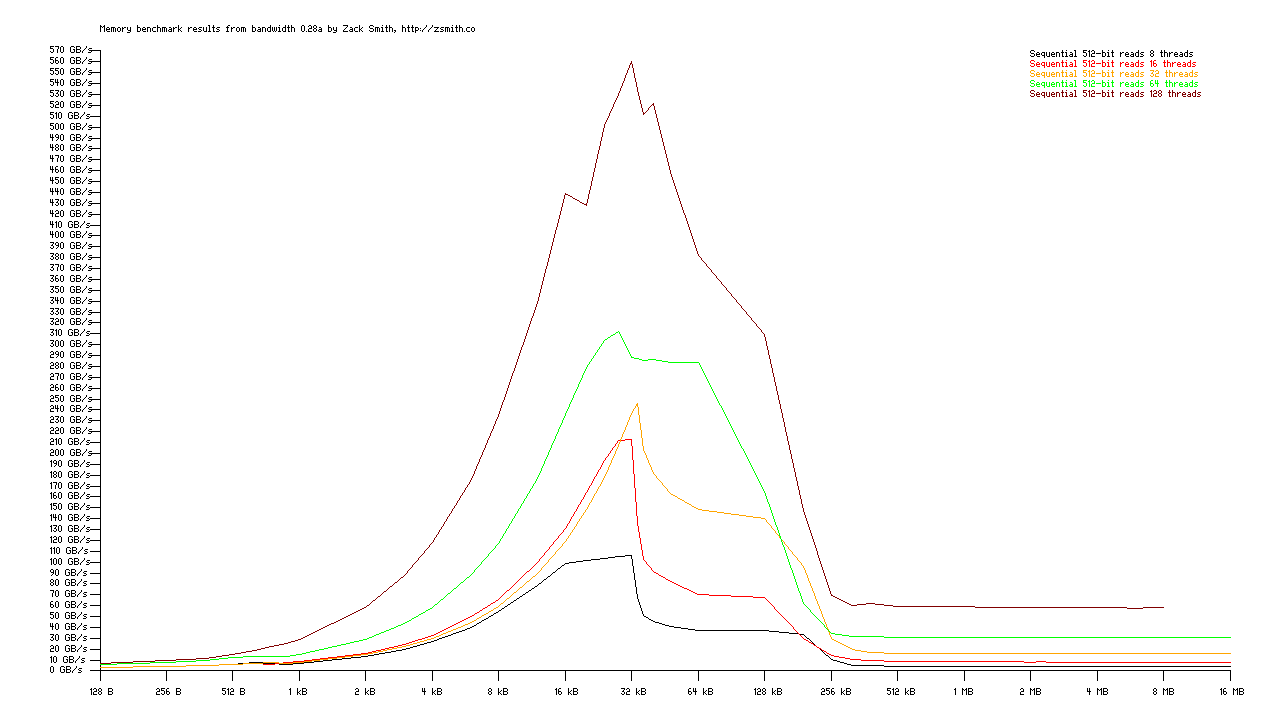
\includegraphics[scale=0.33]{bandwidth_MICO3.png}
					\caption{Bandwidth MIC}
					\end{center}
					\end{figure}
					\begin{figure}
					\begin{center}
					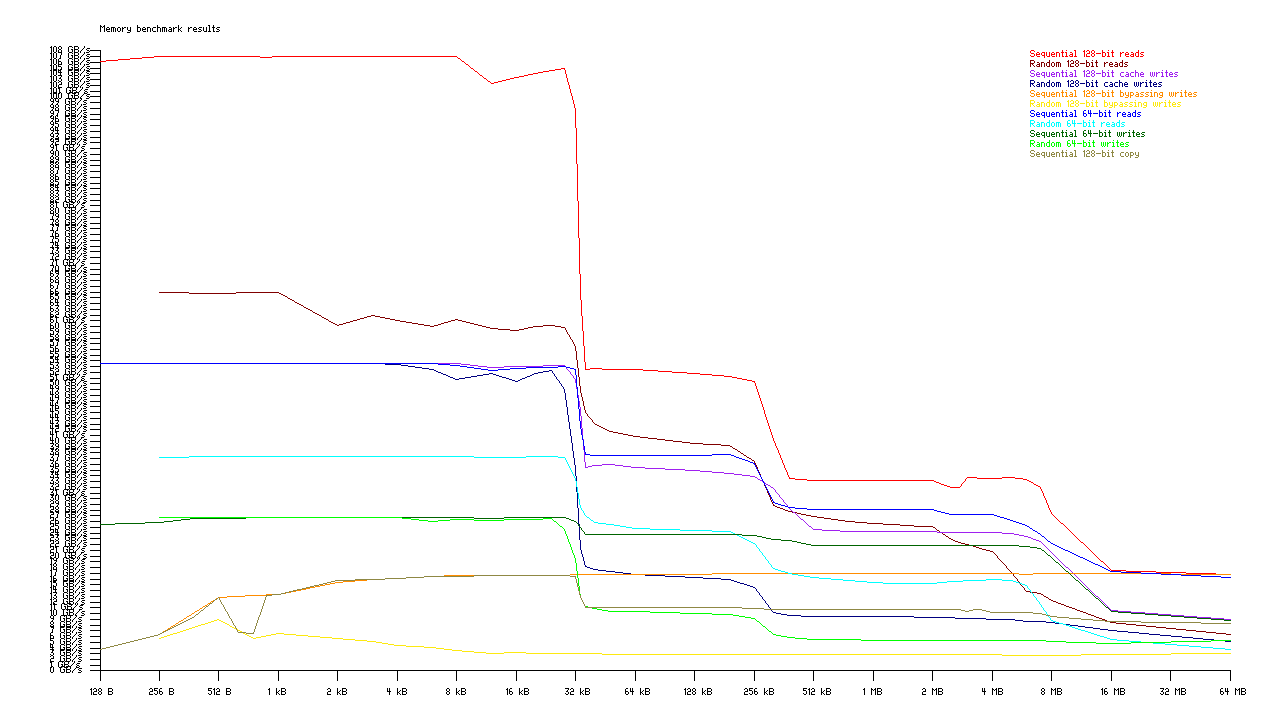
\includegraphics[scale=0.33]{bandwidth_IVYO3.png}
					\caption{Bandwidth Ivy Bridge}
					\end{center}
					\end{figure}
					\subparagraph{}
					Le deuxième métrique que l'on mesure généralement est la latence de la mémoire, à savoir le temps
					nécessaire pour accéder à une mémoire donnée (voir figure 17).
					\begin{figure}[!b]
					\begin{center}
					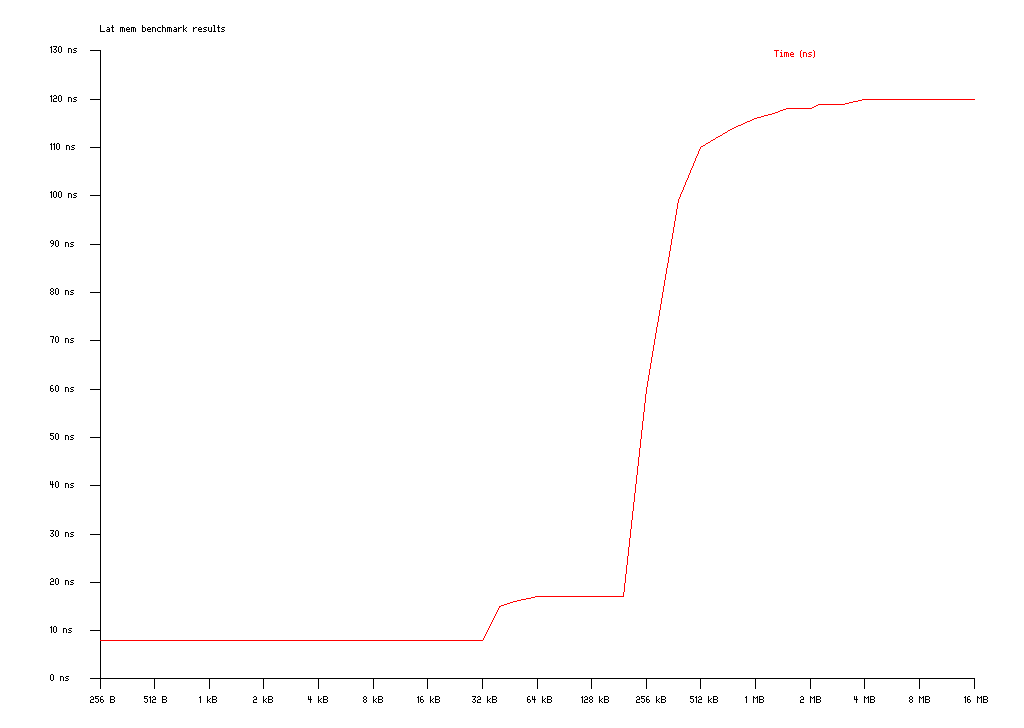
\includegraphics[scale=0.33]{latmem.png}
					\caption{Latence MIC}
					\end{center}
					\end{figure}
				\paragraph{Codes externes}
				Parmi les codes provenant d'organisme client (Ministère de la défense) ou partenaire (CEA), j'ai eu l'occasion 
				de travailler sur deux applications très différentes mais servant de mesure de référence pour évaluer les 
				performances des machines dans des domaines très précis. L'un d'eux réalise des hachages cryptographique et donc
				effectue des opérations sur des nombres entiers, alors que l'autre, est un programme de mécanique des fluide 
				opérant sur des nombres flotants double précision.
					\subparagraph{}
					La fonction de hachage implémentée dans le programme cryptographique, a été portée sur différentes architectures 
					pour tirer partie au mieux des ressources disponibles. Ainsi il existe une version non vectorisée, une version 64 bits (SSE) 
					une version 128 bits (AVX), et une version 256 bits (AVX2). Le MIC travaillant sur des vecteurs 512 bits, 
					il s'agissait donc de créer une version 512 bits et ainsi d'étudier les performances de la carte sur des 
					opérations en nombre entier et de voir si le très grand nombre de coeurs de la carte est profitable à ce 
					type d'algorithme. \newline
					Après avoir compris l'organisation et le fonctionnement du programme, la tâche la plus délicate aura été
					de trouver les informations utiles et nécessaires dans la documentation du MIC. En effet les opérations 
					logiques et arithmétiques sont implémentées avec des intrinsics. Il aura fallu trouver les instructions 
					équivalentes pour MIC et les remplacer (voir figure 18). \newline
					Les tests ont ensuite consistés à comparer les performances en fonction du nombre de coeurs utilisés, et 
					aussi en comparaison avec des processeurs généralistes de type Westmere ou Sandy Bridge.
					\begin{figure}
					\begin{center}
					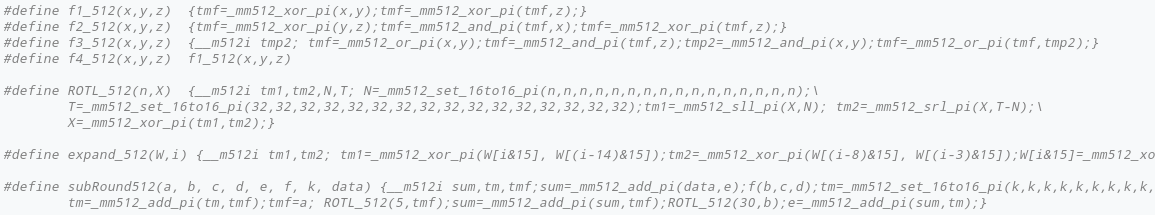
\includegraphics[scale=0.5]{intrinsics.png}
					\caption{Intrinsics MIC}
					\end{center}
					\end{figure}
					\subparagraph{}
					Le code d'Hydro (un programme de calcul de mécanique des fluides) nous a été fourni par le CEA initialement 
					dans le cadre du projet OpenGPU qui sera développé plus tard. Ce code servant à comparer les performances 
					entre CPU et GPU Nvidia, il nous a paru intéressant de le porter également sur MIC et avoir ainsi une 
					comparaison entre trois solutions de calculs différentes sur un code industrielle. \newline
					Deux version du programme existait : \newline
					\begin{itemize}
					\item Une version en C pour CPU
					\item Une version en CUDA pour GPU Nvidia \newline
					\end{itemize}
					Je me suis donc basé sur la version CPU pour faire tout d'abord un portage simple vers le MIC et l'exécuter 
					en mode natif, c'est-à-dire entièrement sur la carte et de manière autonome. Même s'il semblait évident 
					que les performances seraient mauvaises avec ce type d'exécution (OS basique, gestion de la mémoire et des 
					threads, quantité de mémoire) celà permettait néanmoins de vérifier que ce code pourrait fonctionner sur la 
					carte. \newline
					La seconde étape était d'écrire le code à la manière de CUDA, c'est-à-dire en sous-traitant les noyaux de 
					calcul à la carte et en laissant la machine hôte s'occuper de la gestion des entrées-sorties, des fichiers et 
					des allocations mémoires. Il fallait pour cela analyser le code et trouver les point-chauds, autrement dit 
					les parties de code où le programme passe le plus de temps à calculer. Grâce à ses nombreux coeurs de calcul, 
					le Knights Ferry devrait permettre d'accélerer les calculs comparé à un processeur généraliste. Le concept 
					était donc pour les parties de calcul, de transférer les données sur la carte, d'effectuer les calculs sur 
					cette dernière et de renvoyer les résultats vers l'hôte. Malheureusement les résultats n'étaient pas 
					convaincants et même en dégradation comparés à une exécution classique sur CPU. Il y avait plusieurs raisons 
					à celà : \newline
					\begin{itemize}
					\item Tout d'abord la carte étant une version Alpha du produit, comme annoncé par Intel les performances 
					en calcul flotant double précision étaient très mauvaises. Malgré le nombre de coeurs de calcul élevé, 
					la carte était moins rapide qu'une lame Inca 3.
					\item Le seconde raison pour expliquer ces performances est le débit du port PCI-express. En effet le MIC 
					partageait le port PCI-express avec une carte graphique pour l'affichage et le débit était donc deux fois 
					inférieur au débit maximum. Les données transférées entre l'hôte et la carte faisant plusieurs 
					centaines de MégaOctets, un temps considérable était perdu en transfert de données. \newline
					\end{itemize}
					Pour tenter de palier au premier problème, la possibilité de passer les données en simple précision a été 
					implémenté. Les performances se sont alors nettement améliorées, cependant, les temps de transfert restés trop 
					important pour espérer pouvoir être plus performant qu'un GPU, ou même qu'un CPU. \newline
					Les améliorations envisagées pour tenter d'optimiser les transferts n'ont pas abouties, en effet celà aurait 
					nécessité de réécrire de grosses parties du programme et cette option n'etait pas envisageable en temps.
				\paragraph{Outils}
					Jusqu'alors, l'ensemble des développements avaient été fait dans un but d'évaluer les performances du MIC. 
					Afin de s'assurer que le MIC fonctionnait correctement, et pour aller plus loin que les tests fourni par 
					Intel qui se contentaient simplement de vérifier que la carte était reconnue, il m'a été demandé de 
					developper deux tests : \newline
					\begin{itemize}
					\item Un premier test pour évaluer le debit du port PCI-express.
					\item Et un deuxième pour s'assurer qu'aucune erreur n'était introduite lors des transferts entre
					l'hôte et la carte.
					\end{itemize}
					\subparagraph{}
					Encore une fois, plusieurs approches ont été possibles pour réaliser un test de débit du port PCI-express.
					Le procédure globale du test étant de créer un buffer de taille paramétrable, et de l'envoyer de l'hôte 
					vers le MIC, puis du MIC vers l'hôte, et de mesurer le temps qui aura été nécessaire afin de calculer le 
					débit dans chacun des sens. La fonction de mesure du temps utilisée est \emph{gettimeofday}. Cette fonction 
					mesure le nombre de secondes et microsecondes écoulées depuis le 1er Janvier 1970 minuit. Ainsi, en faisant 
					deux appels à cette fonction, l'un au début de la partie à mesurer, et l'autre à la fin, nous pouvons en 
					soustrayant les deux résultats obtenir le nombre de secondes écoulées.\newline
					Ainsi dans la version intiale, l'hôte relevé l'heure lors du début du transfert vers le MIC, et le MIC relevé 
					à son tour l'heure lorsqu'il avait fini de recevoir les données. Seulement voilà, les débits mesurés étaient 
					tous négatifs. La raison à celà : une heure totalement erronée sur l'OS du MIC et surtout différente de celle 
					sur l'hôte. Rien ne pouvant assurer que les deux heures soient identiques, et le test se voulant le plus 
					simple possible à mettre en place, (en évitant de demander à l'utilisateur de configurer l'heure sur le MIC) 
					les mesures ont été faites différemment : \newline
					l'hôte fait toujours appel à \emph{gettimeofday} avant le début des transferts, mais aussi apres les 
					transferts (voir figure 19).
					\begin{figure}
					\begin{center}
					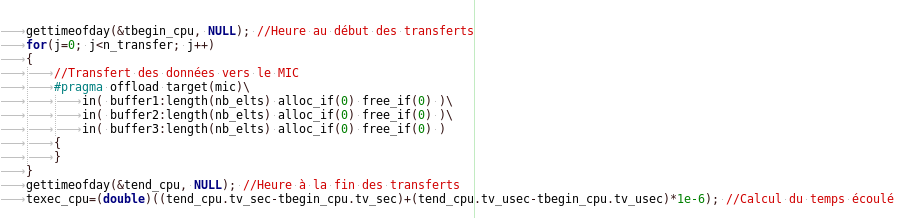
\includegraphics[scale=0.5]{code.png}
					\caption{Mesure temps transfert CPU vers MIC}
					\end{center}
					\end{figure}
					Celà est possible uniquement grâce aux communications asynchrones. C'est-à-dire que l'hôte ne reprend la main 
					sur le programme que lorsque la communication est terminée. Ainsi on est sûr d'avoir relevé l'heure qu'une 
					fois les transferts terminés et pas avant. Enfin le programme est paramétrable, on peut choisir la taille 
					des buffers, le nombre de transfert à effectuer et une limite de temps à ne pas dépasser (voir figure 20).
					\begin{figure}
					\begin{center}
					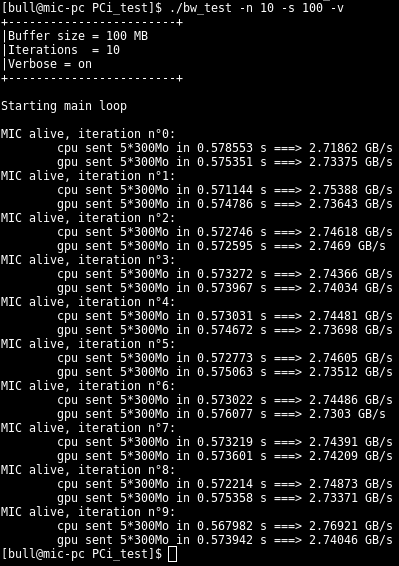
\includegraphics[scale=0.4]{bwtest.png}
					\caption{Mesure débit PCIe avec un buffer de 100Mo, et 10 transferts}
					\end{center}
					\end{figure}
					\subparagraph{}
					Test fiabilité PICe
			\subsubsection{OpenGPU}
			\subsubsection{Knights Corner}
				\paragraph{}
				Knights Corner est le nom donné à la version Beta du MIC. Cette dernière a été mise à disposition par Intel le 2ème trimestre 
				2012. De nombreuses modifications ont été apportés par rapport au Knights Ferry, aussi bien au niveau hardware que software. 
				
			\begin{enumerate}
			\item Knights Ferry
				\begin{itemize}
				\item Lecture de doc (ok)
				\item installation de driver (ok)
				\item Portage de benchmark pour le MIC (ok)
					\begin{itemize}
					\item Bench élémentaire interne à l'équipe (C) (ok)
					\item SpecInt et SpecOMP (perl, C) (ok)
					\end{itemize}
				\item Ecriture de mes propres tests de performances (en cours)
					\begin{itemize}
					\item tests FLOPS pur (assembleur, C) (ok)
					\item portage de DGEMM et SGEMM (C) (ok)
					\item test bande passante (ok)
					\item test latence mémoire (en cours)
					\end{itemize}
				\item Portage code existant
					\begin{itemize}
					\item tsha (assembleur, C) (ok)
					\item Hydro (C) (ok)
					\end{itemize}
				\item Ecriture de doc (wiki) (derniere partie)
				\item Outils
					\begin{itemize}
					\item Test débit port PCIe (C) (ok)
					\item Test fiabilité port PCIe (C) (en cours)
					\end{itemize}
				\end{itemize}
			\item OpenGpu
				\begin{itemize}
				\item Test CPU vs GPU
					\begin{itemize}
					\item Energie
					\item Puissance
					\item Résultats
					\end{itemize}
				\end{itemize}
			\item Knights Corner
				\begin{itemize}
				\item Nouveaux driver ==> nouvelle doc
				\item Même test que pour knights Ferry
				\item Réecriture de certain bout de code:
					\begin{itemize}
					\item tsha
					\item SpecInt \& SpecOMP
					\end{itemize}
				\item Plus de tests dispo sur specInt
				\item Test en mode large pour SpecOMP
				\end{itemize}
			\end{enumerate}
		\subsection{Les tâches périphériques}
			Au cours de mon stage, j’ai pu effectuer deux tâches qui se situent à la périphérie du [•]. Dès lors qu’elles 
			m’ont permis d’apprendre différents aspects de [•], il paraît approprié de s’y attarder. Il s’agit du [•] et 
			de [•] :
	\section{Apports du stage}
		\subsection{Compétences acquises}
			\begin{itemize}
			\item Autonomie.
			\item Travaille en groupe.
			\item Organisation. (Wiki, livrable simple d'utilisation)
			\item Compétences techniques. (debogage, perl, acces distant, GPU)
			\end{itemize}
		\subsection{Difficultés rencontrées et solutions apportées}
		\subsection{La vie en société}
			Mon stage chez [•] a été très instructif. Au cours de ces [•] mois, j’ai ainsi pu observer le fonctionnement 
			d’une [•]. Au-delà, de l’activité de chacun des services, j’ai pu apprendre comment s’articulent les différents 
			départements d’une telle entreprise. Par ailleurs, les relations humaines entre les différents employés de la 
			société, indépendamment de l’activité exercée par chacun d’eux, m’a appris sur le comportement à avoir en toute 
			circonstance.
			\subsubsection{L’articulation des différents départements}
				Comme il a été vu plus haut, [•] départements structurent la société [•]. Aussi, et au travers de l’analyse 
				qui a pu être faite, il apparaît indéniable que tous ces services interviennent à un moment ou a un autre de 
				la prise de décision. Pour autant, cette prise de décision mérite d’être étudiée spécifiquement, dès lors 
				qu’elle est largement [•]. En effet, il est possible de comparer ce type de société [•].
				L’expression la plus éloquente de ce partage de responsabilité est la décision de [•].
				Aussi, toutes les semaines, les [résultats]  étaient diffusés à tous les employés, de manière à ce qu’ils 
				soient impliqués dans les résultats de l’entreprise (sachant que le but est chaque semaine d’avoir un maximum 
				de [•] et à ce qu’ils connaissent [•].
				[La circulation de l’information est ainsi un des points forts que j’ai retenu de cette société, tant au 
				niveau du travail collaboratif, que dans l’implication de tous dans le bon fonctionnement de la société.]
			\subsubsection{Les relations humaines entre les employés}
				Au-delà du fonctionnement de l’entreprise, j’ai pu ressentir [•].
				En effet, l’atmosphère au sein de la société était très [•]. J’ai ainsi constaté que la hiérarchie des 
				fonctions de la société [•] était [•] dans les rapports entre les employés, favorisant par là [•].
				A titre d’exemple, je [•].
				[Au travers de cette convivialité, j’ai pu comprendre que l’activité d’une société est plus performante 
				dans une atmosphère chaleureuse et bienveillante.]
\newpage
\rhead{Conclusion}
\part{Conclusion}
	[La conclusion résume bien sur, dans une première partie, les principales conclusions de votre rapport de stage. Mais la 
	conclusion permet aussi dans une deuxième partie de vous interroger sur la suite, sur l’avenir de l’entreprise, sur le 
	service, et de mettre en perspective votre stage dans votre formation et dans projet professionnel.]
	A titre de conclusion, il semble intéressant de mettre en évidence les questions actuelles qui se posent sur l’avenir de 
	l’industrie de [•], de savoir comment les acteurs économiques vont faire [•]. Au centre de cette question se trouve 
	naturellement le problème de [•]. En effet, mon stage a été très bénéfique à cet égard : [•]. Il en résultera [•]
	La loi du [•] a donné un certain nombre de solutions aux dérives que pourraient prendre le [•]. Pour autant, plutôt 
	que la [•], un changement de [•] apparaît plus à même à régler [•].
	En somme c'etait pas mal!!
\end{document}
